\section{The Activation of Changes}\label{the_activation_of_changes}

\subsection{Overview}\label{sec:activation_overview}
In section \ref{lifecycle}, we have described the lifecycle of a software 
update and there we have seen that once an implementation (UP) is approved, it 
enters the \emph{Activation} phase. This phase is depicted in figure 
\ref{fig:activation_phase_overview}.

\begin{figure}[h!] %[H]
	\centering
	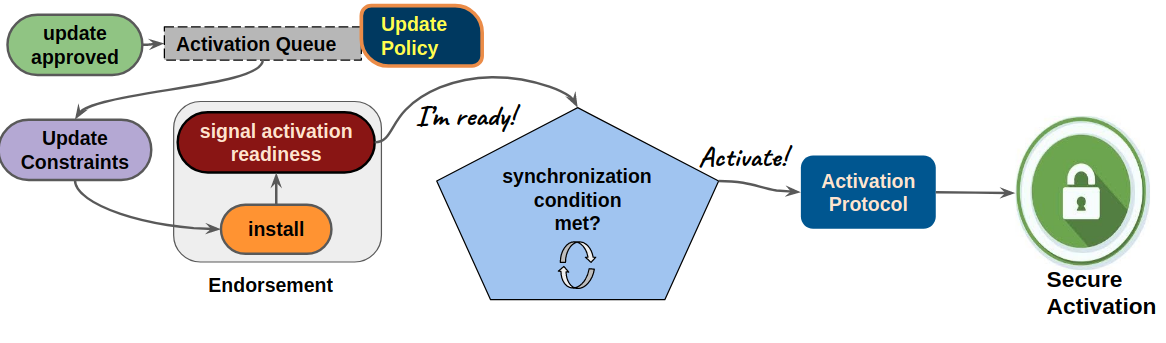
\includegraphics[width=0.8\columnwidth,
	keepaspectratio]{figures/activation_phase.png}
	\caption{The Activation Phase.}
	\label{fig:activation_phase_overview}
\end{figure}

An approved update proposal enters the activation phase and is placed in the
\emph{activation queue}. At this point, the
\emph{update constraints} of the proposal will be evaluated. A proposal
satisfies the update constraints when:
\begin{itemize}
	\item is approved,
	\item meets its dependencies,
	\item does not conflict with the current version,
	\item has the highest priority among competing proposals
\end{itemize}

If a proposal satisfies its update constraints it enters the \emph{Endorsement
Period}. This is the synchronization period discussed in section 	
\ref{se:activation}, where the \emph{block issuers} download and
install the update and \emph{signal upgrade readiness}. We call this signal an 
\emph{endorsement}. Note that only a
\emph{single} proposal can be endorsed at a time. The endorsement period lasts
$N$ number of \emph{epochs}, which is a metadata-defined parameter, called the
\emph{safety lag}; the safety lag corresponds to the sufficient deployment time
window required for the specific update proposal. Once the endorsements reach a
specific stake threshold, called the \emph{adoption threshold}, i.e., when the 
synchronization condition is met, then the activation
gives the green light to the \emph{activation protocol} to run. The activation
protocol ensures the secure activation, i.e., the secure transfer from the old
ledger to the upgraded ledger, based on our formal definition of activation
security and corresponding security proofs \cite{secure_activation}. 

Finally, note that all the metadata-defined information about an update 
proposal, such as the
deployment window length, the proposal's priority, the version dependencies
etc., form the proposal's \emph{update policy} to be followed by the update
system. This policy is accepted and confirmed by the community through the
previous voting process during the Approval phase (see section 
\ref{lifecycle}). In section \ref{activation_phase_design}, we provide details 
on the design of the activation phase.

\ignore {
\subsection{Synchronization for Upgrading} \label{synchronization_for_upgrading}

%\section{Defining a Secure Update System} \label{secureupdate}
We have seen that upon the approval of a UP, users start installing the software update (i.e., upgrade) and wait for the activation of the changes. We call the total  time period from the approval of a UP until the actual activation of the changes in the blockchain system as the \emph{activation lag}. Our protocol should try to minimize this lag and at the same time ensure a secure activation of the changes.

%We call the time period from the approval of a UP until the actual activation of the changes in the blockchain system as the \emph{activation lag}. In order, to enable a fast and flexible software updating mechanism, we should minimize the activation lag, which is in turn is determined by the \emph{adoption threshold} $\tau_A$. %These are the topics to be discussed in this section.

\subsubsection{The Activation of Changes.}\label{se:informal}
%In the lifecycle section, we have described how a software update, after being voted as a SIP, it is submitted again during the approval phase in the form of a UP (source code bundled with metadata), in order to be approved. We make the assumption 
%In our protocol, we assume that if a UP is approved, then sufficient\footnote{\say{sufficient} here means with respect to the resiliency of the new version (i.e., after the upgrade) of the consensus protocol.} (honest) stake will eventually upgrade. However, if we want to have a minimum activation lag, then we cannot wait until all the stake upgrades, to kick-off activation. What is the minimum necessary percent of stake to have upgraded, before the actual activation of the change takes place, in order to avoid a chain split? 
In order to enable a swift and effective update mechanism, we want to minimize the activation lag. 
%What is the minimum necessary percent of stake to have upgraded, before the actual activation of the new softwre takes place, in order to avoid a chain split? 
We need some minimum necessary percent of stake to have upgraded, before the actual activation of the new software takes place that will ensure that a chain split will be avoided. The \emph{adoption threshold} is used in the activation phase and corresponds exactly to the minimum percent of stake that is necessary to have signaled activation readiness, before the actual activation takes place. It is essentially a synchronization point that ensures that a sufficient percent of stake has upgraded and thus it is safe to actually activate the changes. 
%It is therefore a guard against chain splits. 
 Please note that the adoption threshold is only relevant for software updates 
 that impact the consensus protocol. For all other software updates the 
 activation can take place immediately after the upgrade and for protocol 
 parameters it can take place automatically in the next epoch (see on section 
 \ref{se:activation} the discussion about the need for synchronization upon 
 activation).

Let us assume that the adoption threshold of our software update protocol is called $\tau_A$. %In order to enable update policies, we need to be able to adjust $\tau_A$ based on each software update's metadata. 
%What would be the appropriate values for $\tau_A$? 
%\mnote{I noticed that you often pose questions and then answer them as rhetorical device. I am not a fan of this style, so I would suggest to avoid it. But this is just a suggestion based on my personal experience, so feel free to ignore this comment.}
 Intuitively, we would like $\tau_A$ to ensure that a sufficient percent of honest stake will activate, in order for the new version of the blockchain to be secure. Lets assume that $H$ is the percent of honest stake and $T$ is the percent of adversarial stake. From Garay et. al. in \cite{sok}, we know that the ratio $r = \frac{T}{T+H} = \frac{T}{100}$ is upper bounded by the theoretical adversary tolerance $r_{Th}$ of our consensus protocol, i.e., $r = \frac{AdversaryStake}{TotalStake} = \frac{T}{100} < r_{Th}$ (e.g., $r < 1/2 = r_{Th}$, or $r < 1/3 = r_{Th}$ etc.).
%Lets call $r$ the resiliency \footnote{The resiliency in our case is the fraction ($t/n$) of the total adversary stake $t$ to the total stake $n$.}  of the new version of the consensus protocol (i.e., after the activation of changes). $r$ is upper bounded by the theoretical adversary tolerance $r_{Th}$ of our consensus protocol (e.g., $r < 1/2 = r_{Th}$, or $r < 1/3 = r_{Th}$ etc.). So the adversary stake is $r\times100$, while the honest stake is $(1-r)\times100$. 
 Naturally, if we choose $\tau_A \leq H$, then we allow the activation of changes to take place before the minimum required percent of honest stake has the chance to upgrade. Thus, we activate too-early and we risk the security of the new blockchain. 
%partition the honest stake in two and therefore cause a chain split “by accident”

If we consider $\tau_A > H$, then a possible attack would be for the the adversary to rush to signal, so that the threshold $\tau_A$ is met, without sufficient honest stake to have enough time to complete the upgrade. The activation will take place and the new blockchain will run (at least for some time) with an honest stake percent that does not ensure its security. 

In order to prevent this attack, the adoption threshold should be sufficiently 
large, so that the required percent of stake that has signaled will ensure that 
the new blockchain will kick off with sufficient honest stake. It is easy to 
see that in this case, we need $\tau_A \geq \frac{1}{r_{Th}} \times T$, where 
$r_{Th}$ corresponds to the theoretical adversary tolerance of the 
\emph{upgraded protocol} (potentailly different from the original protocol),  
so that for the upgraded stake, the required security property
$\frac{AdversaryStake}{TotalStake_{upgraded}} < r_{Th}$ will still hold and thus the upgraded blockchain will be secure. Indeed, if we assume that the total upgraded stake percent is above the adoption threshold minimum value $\frac{1}{r_{Th}} \times T$ (e.g., $\frac{1}{r_{Th}} \times T + \delta$ where $\delta > 0$) and that all the adversary stake $T$ has upgraded, then if we substitute, we see that the property $\frac{AdversaryStake}{TotalStake_{upgraded}} = \frac{T}{\frac{1}{r_{Th}} \times T + \delta} < r_{Th}$ holds. Therefore, for $T$ percent of adversary stake, the requirement for the adoption threshold is:

\begin{equation} \label{tauA}
\tau_A \geq \frac{1}{r_{Th}} \times T
\end{equation}

For example, if $r_{Th} = \frac{1}{2}$ and we assume that $T = 40\%$, then we will need an adoption threshold of $\tau_A \geq 80\% $, in order to be safe from this attack. However, a too high value of the adoption threshold, one where $\tau_A > H$, introduces another risk; the risk of  giving the opportunity to the adversary to block an activation by refusing to signal. We call this a \emph{Denial of Activation} attack. Intuitively, this blocking problem can be resolved by setting an \emph{activation deadline} ---a time point in the future--- where the activation will take place \emph{regardless} of the adoption threshold condition. To this end, we introduce the concept of the \emph{safety lag}.

%\paragraph{Safety Lag $T_s$}
The safety lag $T_s$ is a metadata-driven artificial delay, which is imposed during the activation phase, in order to give time to the honest stake to upgrade. The safety lag is determined by: 1) the time required to download the software update and 2) the time required to complete the deployment process.
%and 3) sufficient time to ensure that the security assumptions of the new blockchain (after the activation) will hold and that it sufficiently incorporates the old one (before the activation). 
 For example, there might be software updates that entail a very complex deployment process; one that even  a hardware upgrade is required before the software upgrade. In addition, a large software update might require significant time to be downloaded over a slow network connection. In such a case, the safety lag must ensure plenty of time to the stakeholders to upgrade.  
%Similarly, a hard fork type of change, should trigger a greater safety lag than that of a soft fork type of change. 
%We propose both of these to be recorded as important 
We propose that the complexity of the installation process and the size of the software update to be recorded as important characteristics of a decentralized software update's metadata (cf. Appendix \ref{appxmetadata}). This information will drive the choice of the length of the safety lag and enable a metadata-driven update policy.

%Of course the safety lag must also include enough time to ensure that the security assumptions of the new blockchain will hold and that the new blockchain (after the activation) sufficiently incorporates the old one (before the activation).

We propose a synchronization mechanism for the activation phase, which is based on the safety lag and the adoption threshold. Essentially the activation of changes is based on two separate conditions and it is triggered when either of the two comes true: a) Either the adoption threshold is met, based on the above equation, or b) the safety lag period expires. In other words, the safety lag acts as a time upper bound in the case where the adoption threshold is not met. Based on the assumption that given sufficient time %all 
the honest parties will upgrade to an approved software update, the expiration of the safety lag period signifies the case where honest stake has upgraded (based on the assumption that there was sufficient time for this) and the adoption threshold has not been met due to adversary stake blocking. Our protocol breaks this blocking and proceeds to the activation. 

Upon the activation of the changes our protocol ensures that whichever of the two comes first, the new blockchain will be secure and at the same time our update mechanism is protected against the denial of activation attack. We assume that the parties agree on the safety lag by means of a block index. That is, the parties assume that when the $j$-th block 
is generated and becomes a part of the stable part of the blockchain, then there are sufficiently honest parties that have installed the new software and that are ready to run the new code. 
In the following section, we provide a formal description of our activation protocol and of our security proofs. 

\ignore{
Take into account that by adjusting the value of $\tau_A$, we risk to cause a chain split for two distinct reasons: a) A too-low value of $\tau_A$ might result to a \emph{too-early activation}, which will result to the partition of the honest stake in two and a potential chain split\footnote{A partition of the honest stake also undermines the security of the underlying consensus protocol which assumes a minimum threshold $x$ of honest stake.}  and b) a too-high value of $\tau_A$ might result to a \emph{too-late activation}, giving the opportunity to adversaries to block an activation by refusing to signal. We call this a \emph{Denial of Activation} attack. %Clearly the former is a safety problem, while the latter is a security problem. 
What is the allowable range of values for $\tau_A$, in order to mitigate these risks?

In order to avoid both of the two problems described above, the adoption threshold $\tau_A$ should take values in the range $x \leq \tau_A \leq h_a$, where $x$ is the theoretical honest stake threshold of the underlying consensus protocol and $h_a$ is the \emph{actual} percent of honest stake (of course $h_a \geq x$). In addition, we assume that the honest stake that has signaled, when the threshold is met, is at least $x$ ($S_{honest} \geq x$) , i.e., at least equal to the honest stake threshold of the consensus protocol. The rationale of this result is explained in the appendix \ref{appxadoption}, due to space limitations.

A possible attack in the case where $x \leq \tau_A \leq h_a$ is the adversary to hurry to signal for a software update, so that the threshold $\tau_A$ is met, without (at least) $x$ honest stake to have enough time to complete the upgrade (i.e., $S_{honest} < x$). Thus a too-early activation will take place and the honest stake will be partitioned for some time, risking a chain split and also running the consensus protocol without the $x$ honest stake assumption.

Intuitively, in order to prevent this type of attack, we need to give more time to honest stake to upgrade, since we have assumed that all honest stake will eventually upgrade. This is especially true for difficult to deploy software updates, or hard fork type of changes, where the risk of a chain split is greater. A high value of $\tau_A$ would help towards this end, which means that our update policy, would ideally adjust the adoption threshold close to $h_a$ (i.e., to the actual percent of honest stake). Of course, we do not know $h_a$ exactly and we should base it on some sort of estimation. What if we could delay the activation of changes, even though the $\tau_A$ threshold has been met? This is the topic of the next subsection. 
}


%Clients are able to read the ledger
%and submit transactions to be
%added to it.
%The purpose of ledger consensus is to provide a unique
%view to the ledger for the clients. 
%The properties that a ledger consensus protocol must satisfy are as follows:

} % ignore

\import{./}{sections/secure_activation_protocols.tex}

\import{./}{sections/activation_phase_design.tex}
